\documentclass[10pt]{oblivoir}

% ---------------------------------------------- PACKAGE IMPORTS
\usepackage{kotex}
\usepackage{amsmath}
\usepackage{multicol}
\usepackage{fixltx2e}
\usepackage{float}
\usepackage{graphicx}
\usepackage{fullpage}
\usepackage{siunitx}
\usepackage[ruled,vlined]{algorithm2e}
\usepackage{hyperref}
\usepackage{listings}
\usepackage{color}
\usepackage{caption}
\usepackage{indentfirst}
\usepackage{subcaption}
\usepackage{tikz-cd}
\usepackage{chngcntr}
\usepackage{comment}
\usepackage[nameinlink]{cleveref}

% ---------------------------------------------- FIGURE COUNTER SETTINGS
% \counterwithin{figure}{section}

% ---------------------------------------------- CODE AREA SETTINGS
\definecolor{dkgreen}{rgb}{0,0.6,0}
\definecolor{gray}{rgb}{0.5,0.5,0.5}
\definecolor{mauve}{rgb}{0.58,0,0.82}

\lstset{frame=tb,
  language=C++,
  aboveskip=3mm,
  belowskip=3mm,
  showstringspaces=false,
  columns=flexible,
  basicstyle={\small\ttfamily},
  numbers=none,
  numberstyle=\tiny\color{gray},
  keywordstyle=\color{blue},
  commentstyle=\color{dkgreen},
  stringstyle=\color{mauve},
  breaklines=true,
  breakatwhitespace=true,
  tabsize=3
}

% ---------------------------------------------- CLEVERREF SETTINGS
\crefname{figure}{그림}{그림}
\crefname{equation}{식}{식}
\crefname{table}{표}{표}
\crefname{listing}{목록}{목록}
\crefname{section}{절}{절}
\crefname{algorithm}{알고리즘}{알고리즘}

\captionsetup[subfigure]{subrefformat=simple,labelformat=simple}
    \renewcommand\thesubfigure{ (\alph{subfigure})}

% ---------------------------------------------- GENERAL SETTINGS
\setlength{\parindent}{0.3cm} % The first indent width setup

% ---------------------------------------------- CUSTOM COMMANDS
%       GENERAL
\newcommand{\textss}[1]{\scriptsize#1\normalsize}
%       MATHEMATICAL
\newcommand{\abs}[1]{\left|\,#1\,\right|}

% ---------------------------------------------- HEADER
\title{AR 당구 개선 진행 상황 보고}
\author{강승우}
\date{2020.11.27}

% ---------------------------------------------- CONTENT
\begin{document}
\maketitle

\section{인터페이스 개선 사항}
영상 인식 프로그램에 파이프라인 구조를 도입(\cref{fig;interface}), 영상 처리의 의존적이지 않은 각 단계를 분리하여 병렬적으로 실행될 수 있게 하였습니다. 파이프 하나당 오버헤드는 5~ 10us 정도로, 전체 프로세스에서 차지하는 비중은 미미한 편입니다.

\begin{figure}[ht]
    \centering
    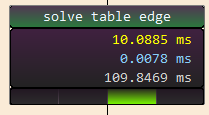
\includegraphics{img/pipe.png}
    \caption{위에서부터 지연, 알고리즘 실행, 출력 인터벌 시간, 하단의 초록색 바는 현재 파이프의 각 실행기 상태}
\end{figure}

이를 통해 알고리즘 자체가 다소 비효율적이더라도, 다수의 파이프를 병렬로 분산 배치하여 출력 사이의 인터벌을 N배수로 감소시킬 수 있게 되었습니다. (단, 첫 입력부터 출력까지의 지연 시간 감소에는 알고리즘의 효율화가 필요합니다)

\begin{figure}[ht]
    \centering
    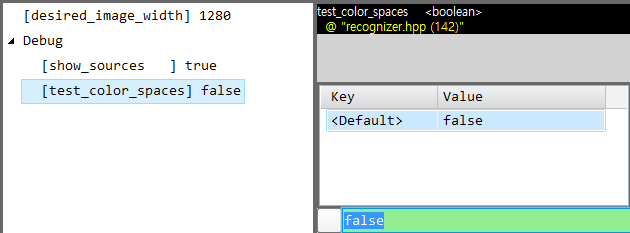
\includegraphics{img/options.png}
    \caption{}
    \label{fig;option-view}
\end{figure}
    
개발 과정 중 파이프의 여러 가지 상수 파라미터를 정의하는 함수성을 다수 추가하였으며, 이를 그래픽 인터페이스를 통해 손쉽게 조작하고 확인할 수 있습니다(\cref{fig;option-view}).

\begin{figure}[ht]
    \centering
    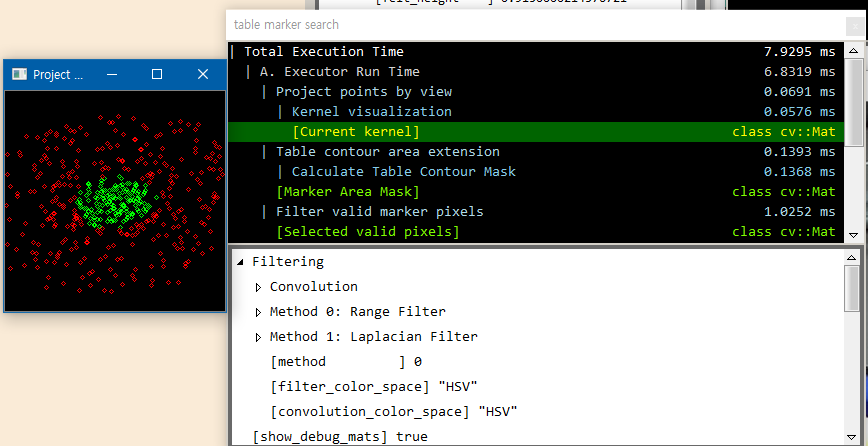
\includegraphics[width=15cm]{img/pipe-view.png}
    \caption{}
    \label{fig;pipe-view}
\end{figure}

또한, 각 파이프의 알고리즘 실행 도중 각 알고리즘의 실행 시간 및, 디버깅을 위해 모니터링이 필요한 정보들을 gui 프레임에서 실시간으로 확인할 수 있게 하였습니다(\cref{fig;pipe-view}). 

\begin{figure}[H]
    \centering
    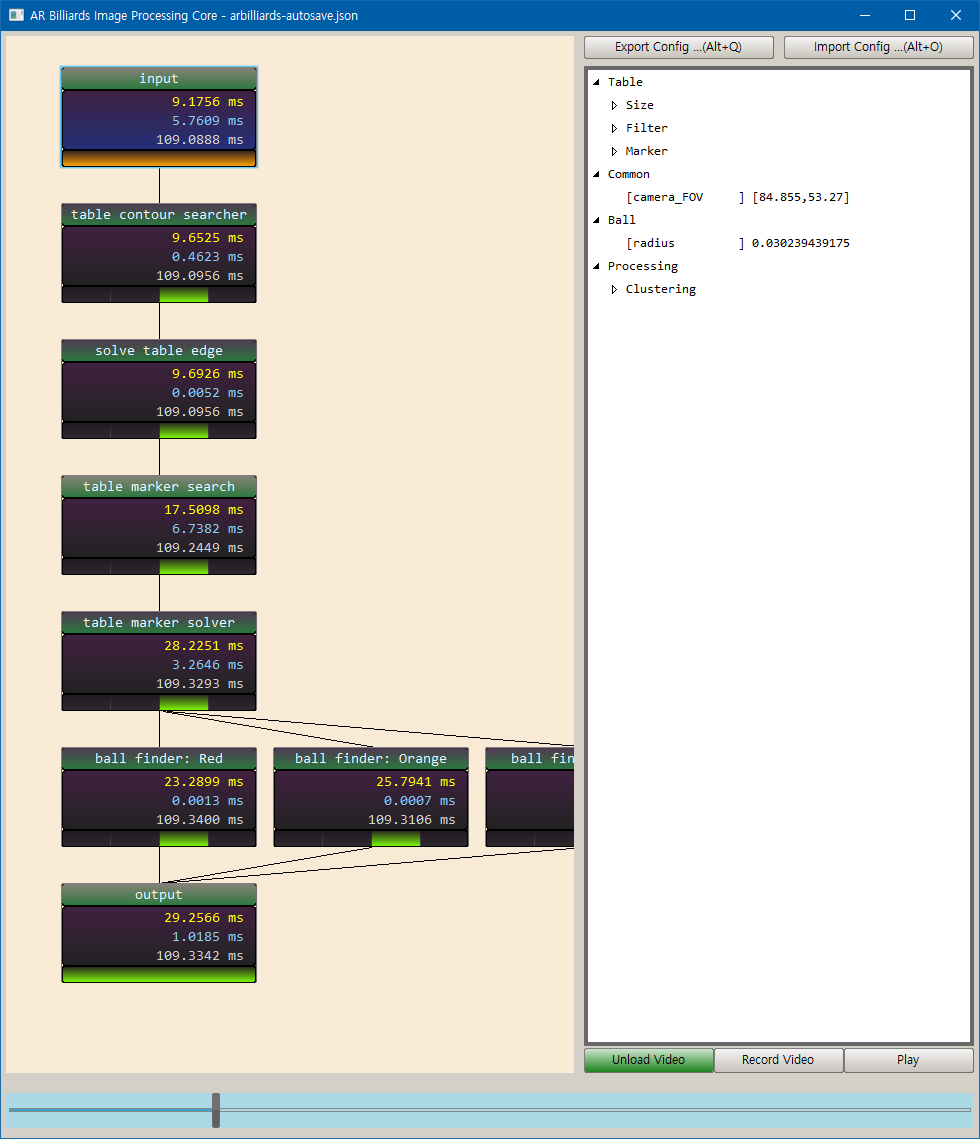
\includegraphics[width=18cm]{img/interface.png}
    \caption{}
    \label{fig;interface}
\end{figure}

\section{알고리즘 개선 사항}

당구대의 각 마커 포인트 인식 알고리즘을 대폭 개선했습니다. 기존의 알고리즘은 단순히 경계선 필터를 적용하고 thresholding을 통해 검출된 영역의 contour 중점을 추출하는 식이었지만, 새로 개선한 알고리즘은 이전에 소개드린 희소 커널 콘볼루션을 적용하여 더 정확하게 마커 위치를 평가합니다.

방법은 다음과 같습니다.

\begin{figure}[ht]
    \centering
    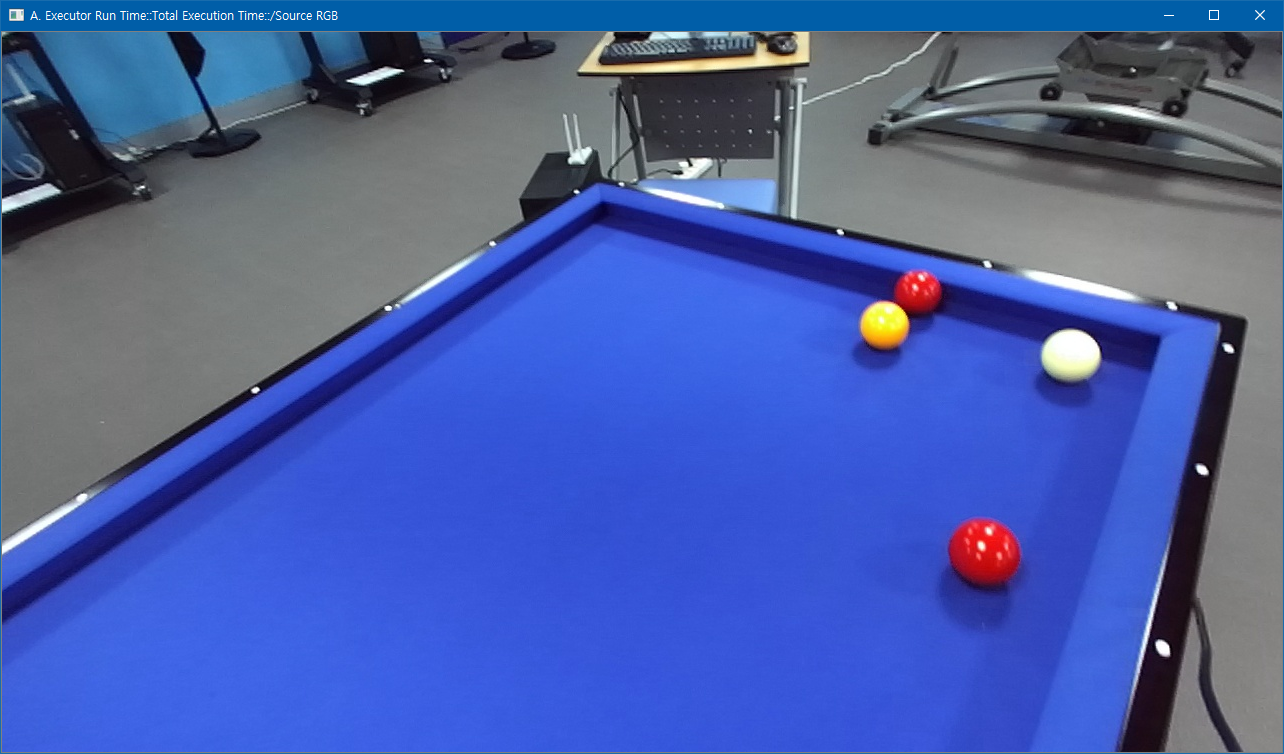
\includegraphics[width=12cm]{img/sample-view.png}
    \caption{}
    \label{fig;sample-0}
\end{figure}

\begin{figure}[ht]
    \centering
    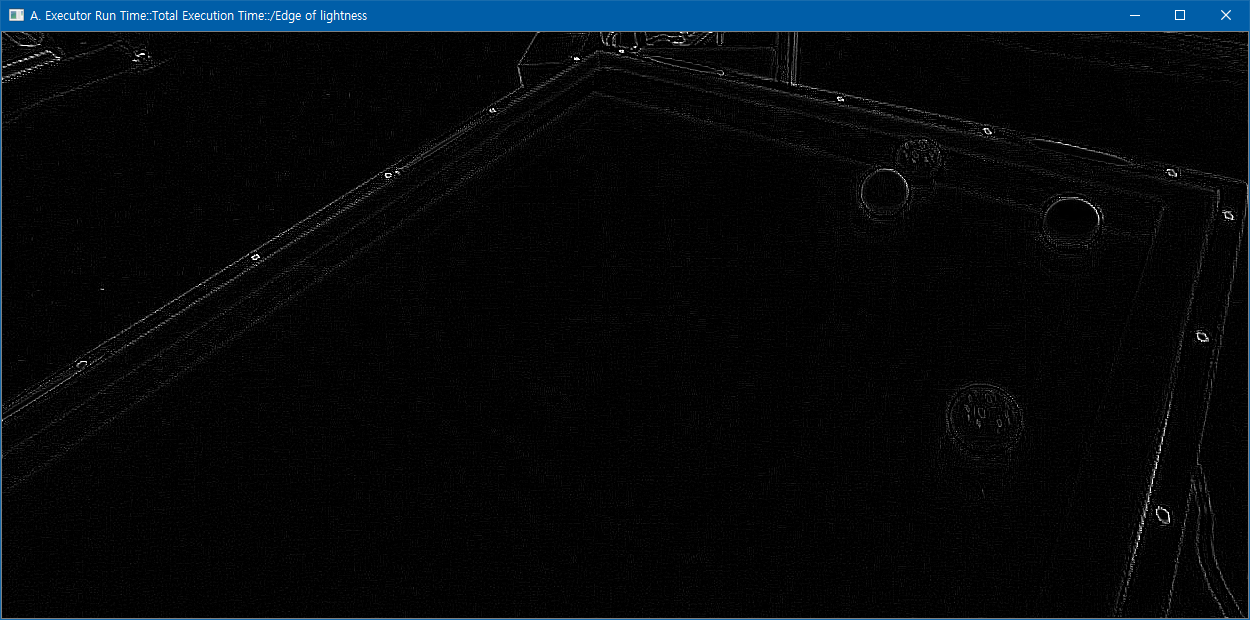
\includegraphics[width=\textwidth]{img/sobel.png}
    \caption{기존 방법: 경계선 검출 필터}
    \label{fig;old-edge}
\end{figure}

\cref{fig;sample-0}과 같은 환경에서, 기존의 경계선 기반 검출 알고리즘은 \cref{fig;old-edge}와 같이 경계선을 검출하고, 이를 thresholding 해 직접 마커 위치로 삼았기 때문에 잡음이 매우 심했으며, 색상을 평가하지도 않았기 때문에 올바른 결과를 보장하지 않았습니다.

\begin{figure}[ht]
    \centering
    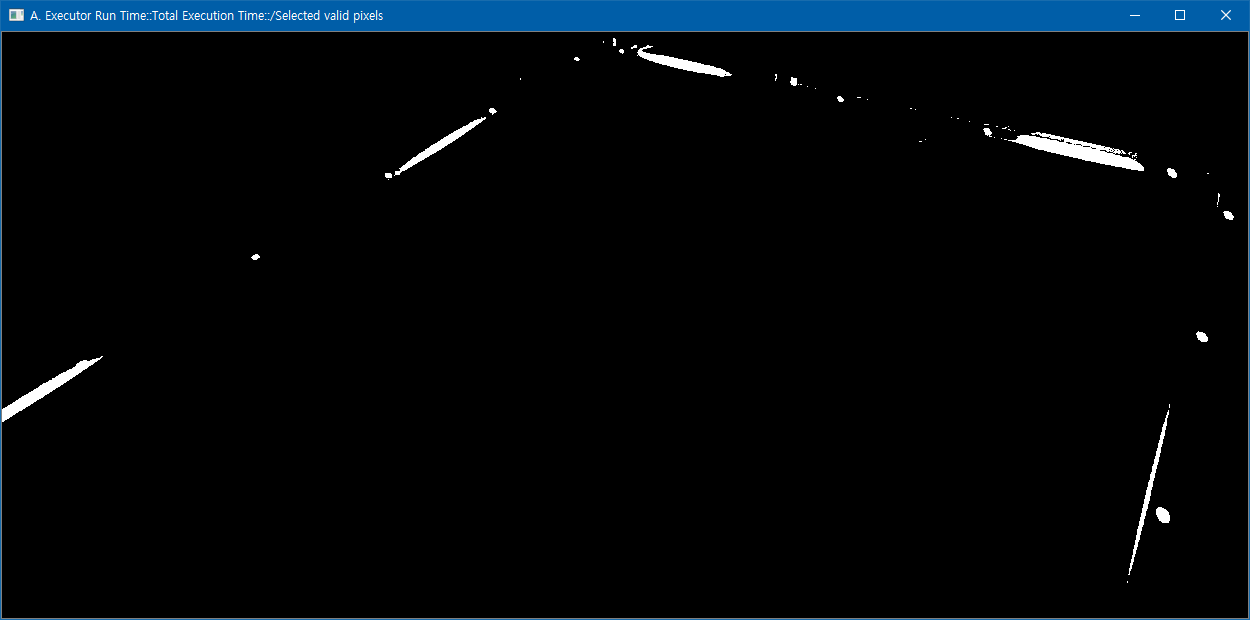
\includegraphics[width=12cm]{img/new-pp0.png}
    \caption{단순히 흰색에 가까운 모든 픽셀을, 다소 보수적인 범위에서 필터링합니다}
    \label{fig;new-pp0}
\end{figure}

새로운 방법은 위에서 검출된 먼저 단순한 범위 기반 필터를 적용하여 얻어진 \cref{fig;new-pp0}의 점 각각을 마커의 추정 중점으로 삼고, 이전에 공 검출에서 사용된 바 있는 가변 크기의 희소 커널 컨볼루션을 적용합니다. 그러나 공과 달리 마커는 평면 상에 위치하기 때문에 테이블과 시야가 이루는 각도에 따라 모양이 달라지므로, 희소 커널의 원형을 3D 공간에 배치한 후 매 프레임마다 시야에 대한 테이블의 상대 각도로 트랜스폼을 적용합니다.

\begin{figure}[ht]
    \centering
    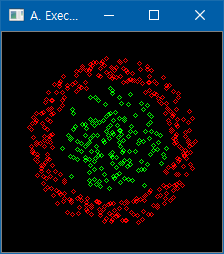
\includegraphics[width=6cm]{img/kernel-source.png}
    \caption{희소 커널의 원형}
    \label{fig;kernel-src}
\end{figure}

희소 커널의 원형은 \cref{fig;kernel-src}와 같습니다. 초록색 영역에 해당하는 점은 양의 적합도로 평가되며, \cref{fig;new-pp0}의 흰색 넓은 영역이 마커로 평가되지 않게끔 빨간색 영역에 해당하는 점은 적합도가 음의 가중치로 평가됩니다.

그러나 \cref{fig;sample-0}에서도 볼 수 있듯 평면상의 마커는 시야에 따라 그 각도가 달라지기 때문에, 매 프레임 커널의 각도를 재계산해 1 meter 거리에 투영, 이를 커널의 원형으로 사용합니다.

\begin{figure}[ht]
    \centering
    \begin{subfigure}{0.3\textwidth}
        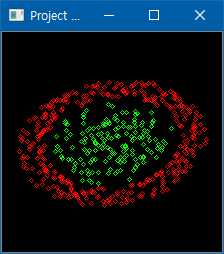
\includegraphics[width=\textwidth]{img/kernel-project-0.png}
    \end{subfigure}
    \begin{subfigure}{0.3\textwidth}
        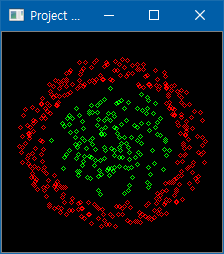
\includegraphics[width=\textwidth]{img/kernel-project-1.png}
    \end{subfigure}
    \begin{subfigure}{0.3\textwidth}
        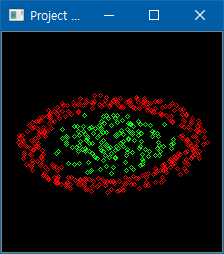
\includegraphics[width=\textwidth]{img/kernel-project-2.png}
    \end{subfigure}
    \caption{다양한 각도로 투사된 커널}
\end{figure}

또한 sparse kernel convolution에 GPU 연산(C++ AMP 사용)을 도입하여, 기존에 20ms 가까이 걸리던 연산 시간을 샘플 개수에 거의 관계없는 2ms 수준으로 낮출 수 있었습니다.

\begin{figure}[ht]
    \centering
    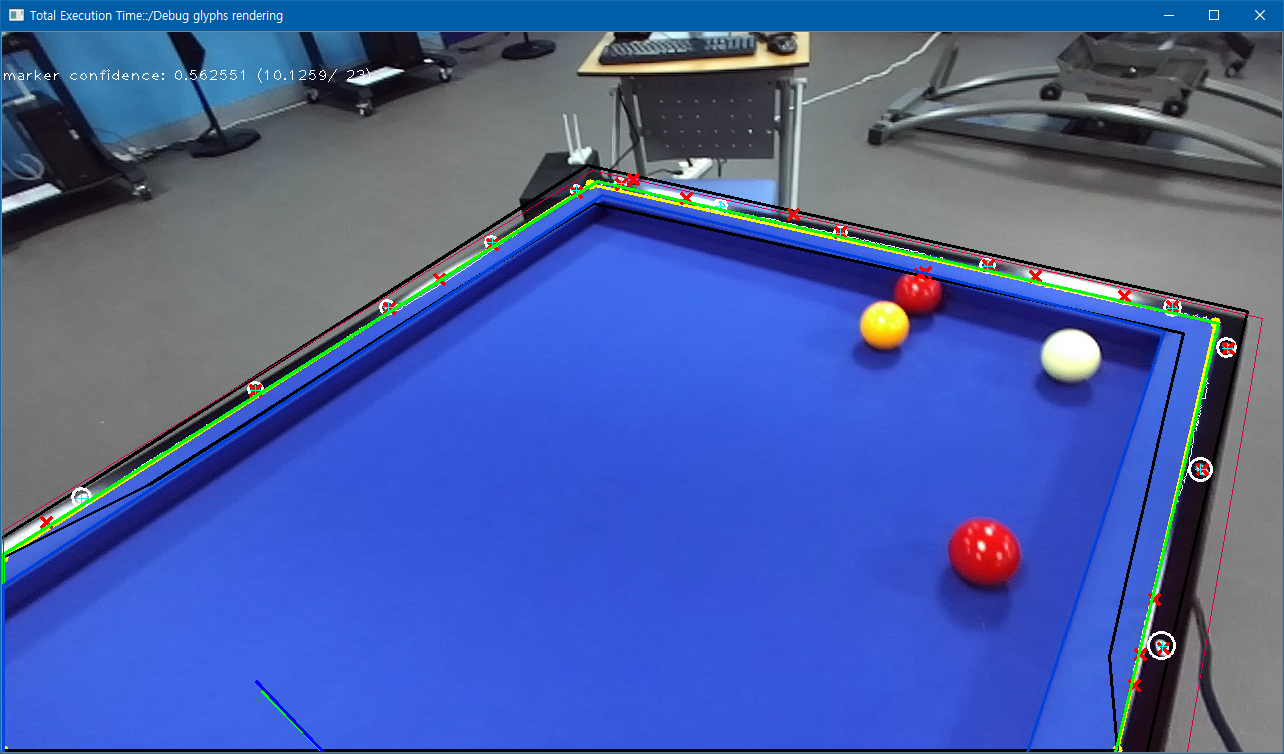
\includegraphics[width=\textwidth]{img/result.png}
    \caption{인식 결과. 빨간색 가위표는 마커로 인식된 위치이며, 흰색 동그라미는 계산된 테이블 위치에 따라 마커의 추정 위치를 투사한 것입니다}
    \label{fig;result}
\end{figure}

그 결과 \cref{fig;result}에서와 같이 비교적 안정적인 마커 위치를 획득할 수 있습니다. (마커 위치 기반의 solve는 어느 정도 노이즈에 둔감하게끔 설계해서, 그림에 보이는 몇 개의 노이즈는 무시할 수 있는 수준입니다)

지금까지 개선된 부분은 이 정도이며, 공 탐색 알고리즘 또한 조명의 위치를 바탕으로 일종의 셰이더를 수행해 정확한 커널을 획득, 가변 템플릿 매칭을 구현할 계획입니다.

\section{향후 계획}

현재 물리 시뮬레이션에 PhysX 엔진을 도입하여 시뮬레이션 퀄리티를 높일 계획을 하고 있습니다. 그러나 이 경우 연산량이 많아 기존처럼 수백~수천 개의 케이스를 10초 단위 길이로 시뮬레이션하기는 어려울 듯하여, 머신 러닝을 실험적으로 도입해 보려 하고 있습니다. 

\begin{figure}[H]
    \centering
    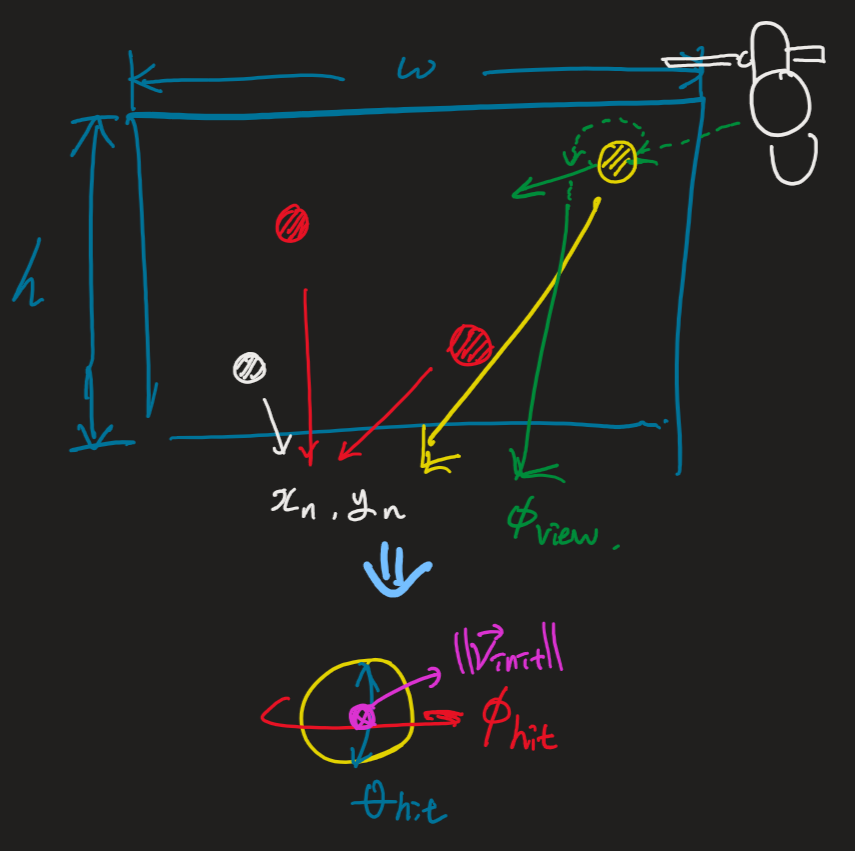
\includegraphics[width=\textwidth]{img/params.png}
    \caption{공의 배치와 사용자의 시야 방향을 토대로, 공의 당점과 타격 방향을 결정}
    \label{fig;params}
\end{figure}

현재 갖고 있는 아이디어는 \cref{fig;params}와 같습니다. 각 공의 위치 x, y와 사용자의 시야 방향(가급적 정면의 경로를 추천하도록)을 합한 9개 차원에서, 공을 어느 속도($\vec{v}_{(init)}$)로, 어떻게 당점($\phi_{(hit)}, \theta_{(hit)}$)을 주어 타격하면 득점할 수 있는지를 반환하는 것입니다.

PhyX 시뮬레이터를 사용하면 무수한 양의 훈련 데이터를 노이즈 없이 얻을 수 있으므로, 일단은 괜찮지 않을까 싶습니다.

지금은 일단 SVM으로 다변량 회귀 모델을 구축하려고 생각하고 있는데, 제가 아직 지식이 얕아서 어떻게 될지는 잘 모르겠습니다 ....

여건이 되면 강화학습 모델을 실험해보고 싶지만, 그러기 위해서는 python의 tensorflow 런타임과 c++의 physX 런타임을 연결할 인터페이스를 구현해야 하기 때문에, 시간 관계상 신중하게 결정해야 할 것 같습니다.


\end{document}
